\documentclass[book.tex]{subfiles}
\begin{document}
\label{chapter_software_architecture}
\section{About the Source Code}
Commander Keen episodes 1-5 source code is unavailable, as the current owner Zenimax\footnote{June 24, 2009, it was announced that id Software had been acquired by ZeniMax Media (owner of Bethesda Softworks).} has, at the time of writing, shown no interest in selling the intellectual property. Luckily the ownership of Commander Keen: Keen Dreams was in the hands of Softdisk. In June 2013, developer Super Fighter Team licensed the game from Flat Rock Software, the owners of Softdisk at the time, and released a version for Android devices.\\

\par
The following September, an Indiegogo crowdfunding campaign was started to attempt to buy the rights from Flat Rock for US\$1500 in order to release the source code to the game and start publishing it on multiple platforms. The campaign did not reach the goal, but it’s creator Javier Chavez made up the difference, and the source code was released under GNU GPL-2.0-or-later soon after.


\section{Getting the Source Code}
The source code is available on \cw{github}. It is essential to use the source code from the shareware version 1.13, or you may encounter issues due to incompatible map and graphs headers\footnote{See issue \#7 on https://github.com/keendreams/keen.}. To get the correct source code, use the following commands in the console \\

\par
\tcode{keen13_github.txt}\\

\section{First Contact}
After downloading the repository from \cw{github}, a folder named 'keen' is created, containing all the source files. The \cw{cloc.pl} tool can be used to analyze the folder and generate statistics about the source code. This tool is useful for getting an idea of what to expect.\\

\par
\begin{minipage}{\textwidth}
\lstinputlisting[]{code/cloc.txt}
\end{minipage}

\par
Approximately 85\% of the code is in C, with assembly\footnote{All the assembly in Keen is done with TASM (a.k.a Turbo Assembler by Borland). It uses Intel notation where the destination is before the source: \cw{instr} \cw{dest} \cw{source}.} used for bottleneck optimizations and low-level I/O operations such as video and audio handling. \\

\par
Source lines of code (SLOC) are not particularly meaningful for comparing a single codebase but are helpful for determining the proportion of code in various components. Commander Keen has 19,237 SLOC, which is small compared to most modern software. For instance, \cw{curl} (a command-line tool for downloading URLs) has 154,134 SLOC, Google Chrome has 1,700,000 SLOC, and the Linux kernel consists of 15,000,000 SLOC.\\

\par
\begin{figure}[H]
\centering
  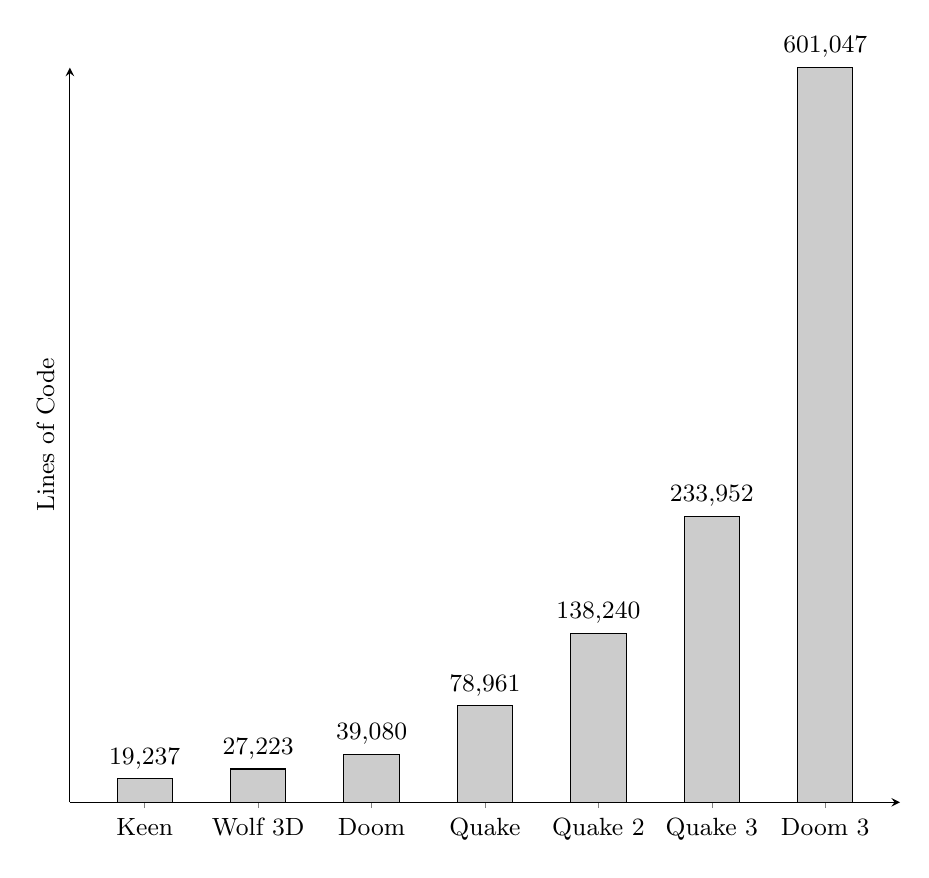
\begin{tikzpicture}[font=\small]
    \begin{axis}[
      width=\textwidth,
      height=0.9\textwidth,
      ybar=0.6\textwidth,
      bar width=20pt,
      ylabel={Lines of Code},
      ymin=0,
      ytick=\empty,
      xtick=data,
      axis x line=bottom,
      axis y line=left,
      enlarge x limits=0.11,
      symbolic x coords={Keen, Wolf 3D,Doom,Quake,Quake 2,Quake 3, Doom 3},
      xticklabel style={},
      yticklabel style={},
      nodes near coords={\pgfmathprintnumber[fixed,precision=0]\pgfplotspointmeta}
    ]
      \addplot[fill=black!20,draw=black] coordinates {
        (Keen, 19237)
        (Wolf 3D,27223)
        (Doom,39080)
        (Quake,78961)
        (Quake 2, 138240)
        (Quake 3, 233952)
        (Doom 3, 601047)
      };
    \end{axis}
   \end{tikzpicture} 
   \caption{Lines of code from id Software game engines.}
 \end{figure}
 
\par


 
The archive contains more than just source code; it also features:
\begin{itemize}
\item A \cw{static} folder with static header files for loading assets (as explained in Section \ref{section:graphic_assets}).
\item An \cw{lscr} folder for loading and decompressing Softdisk data files.
\item A \cw{README} file explaining how to build the executable.
\end{itemize}

\pagebreak
\section{Compile source code}
Now let's start to compile the source code. To compile the code like it's 1990 you need the following software:
\begin{itemize}
\item Commander Keen source code.
\item DosBox.
\item The Compiler Borland C++ 3.1.
\item Commander Keen: Keen Dreams 1.13 shareware (for the assets).
\end{itemize}

\par
After setting up DOSBox and installing Borland C++ 3.1\footnote{you can find a complete tutorial in "Let's compile like it's 1992" on fabiensanglard.net}, download the source code from github.\\

\par
Once DOSBox is running and you've navigated to the \cw{keen} folder, create a folder to store your compiled object files. \\

\par
\tcode{mkdir.txt}\\
\par
Then, generate the static \cw{OBJ} header files.\\
\par
\tcode{static.txt}\\
\par
After that, return to the \cw{keen} folder and open Borland C++. Open the \cw{kdreams.prj} project file. Before compiling, adjust the directory settings by selecting Options -> Directories and change the values as shown on the next page. \\

\par
Now it's time to compile. Go to Compile -> Build All, and voil\`a! The final step is to copy \cw{kdreams.exe} into the Keen shareware folder. ou can now play your compiled version of \textit{Commander Keen}. \\

\begin{figure}[H]
\centering
  \fullimage{borland_directories.png}
  %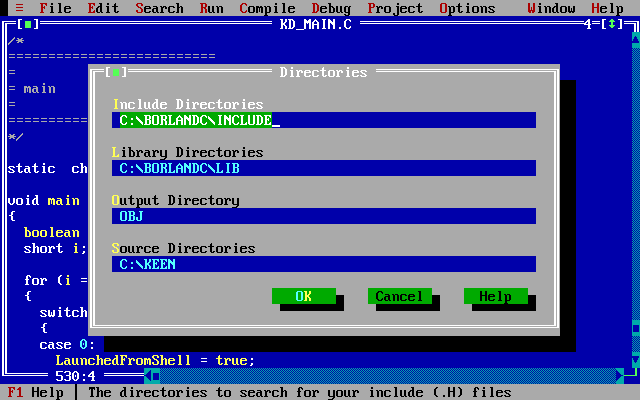
\includegraphics[width=\textwidth]{screenshots_300dpi/borland_directories.png}
%\caption{Borland C++ 3.1 directory settings}
\end{figure}

 \begin{figure}[H]
\centering
  \fullimage{borland_compile.png}
%\caption{Borland C++ 3.1 directory settings and compiling}
\end{figure}


\section{Big Picture}
The game engine is divided in three blocks:
\begin{itemize}
\item Control panel which lets users configure and start the game.
\item 2D game renderer where the users spend most of their time.
\item Sound system which runs concurrently with either the Menu or 2D renderer. 
\end{itemize}
The three systems communicate via shared memory. The renderer writes sound requests to the RAM (also making sure the assets are ready). These requests are read by the sound "loop". The sound system also writes to the RAM for the renderers since it is in charge of the heartbeat of the whole engine. The renderers update the screen according to the wall-time tracked by \cw{TimeCount} variable.
\par
\begin{figure}[H]
\centering
 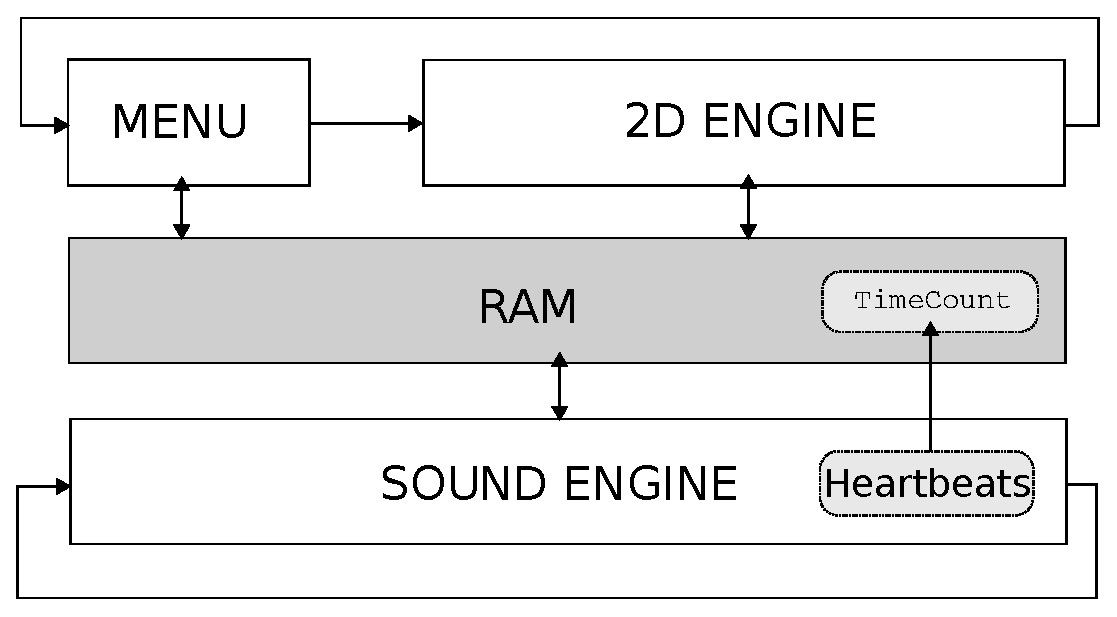
\includegraphics[width=0.95\textwidth]{imgs/drawings/three_systems.eps}
 \caption{Game engine three main systems.}
 \end{figure}
 \par
 
\subsection{Unrolled Loop}
With the big picture in mind, we can dive into the code and unroll the main loop, starting with \cw{void main()}. The control panel and 2D renderer follow regular loops, but due to limitations discussed later, the sound system is interrupt-driven and therefore operates outside the main loop. In real mode, C types do not behave as expected on a 16-bit architecture.
\begin{itemize}
\item \cw{int} and \cw{word} are 16 bits.
\item \cw{long} and \cw{dword} are 32 bits.
\end{itemize}
\par
The first action taken by the program is to set the text color to light grey and the background to black. \\
\par
\begin{minipage}{\textwidth}
\lstinputlisting[language=C]{code/unrolled_loop_main.c}
\end{minipage}
\par

\par
In \cw{InitGame()}, the program checks whether there is enough memory and brings up all the managers.\\
\par
\begin{minipage}{\textwidth}
\lstinputlisting[language=C]{code/unrolled_loop_init.c}
\end{minipage}
\par
Then comes the core loop, where the menu and 2D renderer are called forever.

\begin{minipage}{\textwidth}
\lstinputlisting[language=C]{code/unrolled_loop_demoloop.c}
\end{minipage}
\par
\cw{PlayLoop} contains the 2D renderer. It is pretty standard with getting inputs, update screen, and render screen approach.\\
\par
\begin{minipage}{\textwidth}
\lstinputlisting[language=C]{code/unrolled_loop_playloop.c}
\end{minipage} \\
\par
 
The interrupt system is started via the Sound Manager in \cw{SDL\_SetIntsPerSec(rate)}. While there is a famous game development library called Simple DirectMedia Layer (SDL), the prefix \cw{SDL\_} has nothing to do with it. It stands for SounD Low level (Simple DirectMedia Layer did not even exist in 1990).\\
\par
The reason for interrupts is extensively explained in Chapter \ref{audio_and_heartbeat} "\nameref{audio_and_heartbeat}". In short, with an OS supporting neither processes nor threads, it was the only way to have something execute concurrently with the rest of the engine.\\
\par
An ISR (Interrupt Service Routine) is installed in the Interrupt Vector Table to respond to interrupts triggered by the engine. \\
\par
\begin{minipage}{\textwidth}
\lstinputlisting[language=C]{code/soundsystem_interrupt.c}
\end{minipage}
\par



\pagebreak
\section{Architecture}

The source code is structured in two layers. KD\_* files are high-level layers relying on low-level ID\_* sub-systems called Managers interacting with the hardware.\\
\par
\begin{figure}[H]
\centering
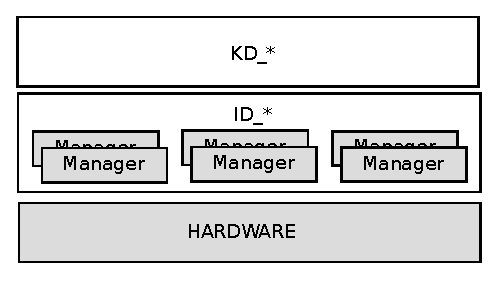
\includegraphics[width=\textwidth]{imgs/drawings/layers.eps} 
\caption{Commander Keen source code layers.}
 \end{figure}
 \par
There are six managers in total:\\

\begin{itemize}
	\item Memory
	\item Video
	\item Cache
	\item Sound
	\item User
	\item Input
\end{itemize}
\par
The KD\_ stuff was written specifically for Commander Keen while the ID\_ managers are generic and later re-used (with improvements) for newer ID games (Hovertank One, Catacomb 3-D and Wolf3D).

\begin{figure}[H]
\centering
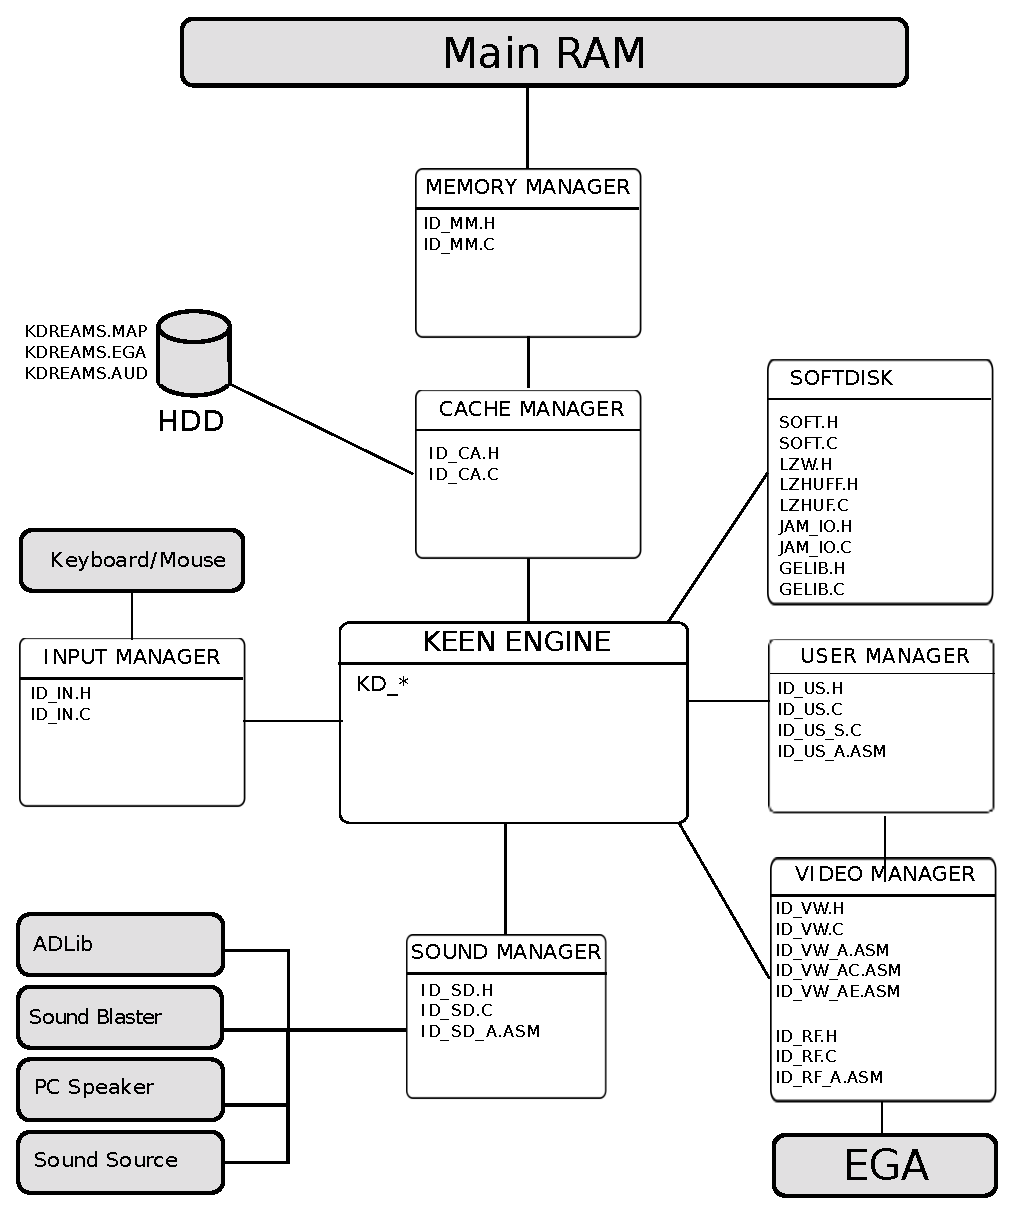
\includegraphics[width=\textwidth]{imgs/drawings/architecture.eps}
\caption{Architecture with engine and sub-systems (in white) connected to I/O (in gray).}
\label{fig:architecture}
\end{figure}
Next to the hard drives (HDD) you can see the assets packed as described in Chapter \ref{section:graphic_assets}.



\subsection{Memory Manager (MM)}
The engine has its own memory manager, to have more control over memory fragmentation and optimization. The memory manager is made of a linked list of "blocks" keeping track of the RAM. A block points to a starting point in RAM, has a size and can be marked with attributes:
\begin{itemize}
  \item LOCKBIT : This block of RAM cannot be moved during compaction.
  \item PURGEBITS : Two levels available, 0= unpurgeable, 3=purge first.
\end{itemize}

\par
\lstinputlisting[language=C]{code/mm_block.c}
\par  
The memory manager allocates all RAM, starting from \cw{00000h}, and assigns segments to the linked list. Since the engine is compiled using the medium memory model, there are two heaps: the near heap between the global variables and stack, and the far heap starting right behind the stack . The total available free memory space for the near heap can be obtained by\\
\par
\lstinputlisting[language=C]{code/nearheap.c}

\par  
The memory manager is segment-aligned, meaning it allocates memory blocks in chunks of 16 bytes. Therefore, the start and length of the memory block must be segment aligned. \\


\lstinputlisting[language=C]{code/mm_block_first.c}

\par  
The first block allocated is the unusable memory from segment \cw{0000h} to the start of the near heap.\\


\lstinputlisting[language=C]{code/mm_getnewblock.c}
\par  

\begin{figure}[H]
\centering
 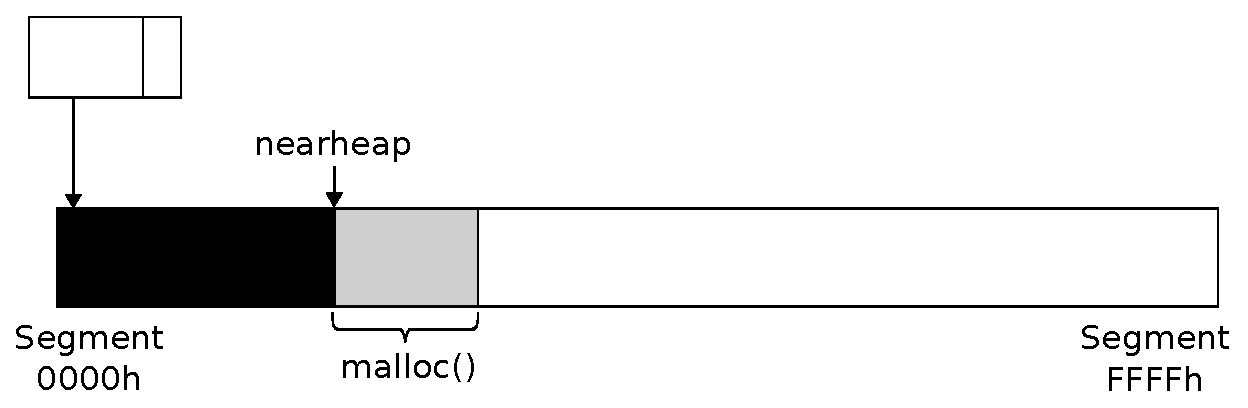
\includegraphics[width=\textwidth]{imgs/drawings/mm_start.eps}
 \caption{First locked block of unusable memory.}
 \end{figure}
 \par

\par
The stack is the next unusable memory block. Since the stack will grow or shrink during game execution, an additional part of the near heap’s free memory must be reserved for it.\\

\par
\lstinputlisting[language=C]{code/mm_savenearheap.c}
\par  

The next step is allocate the far heap, which can be obtained by\\

\par
\lstinputlisting[language=C]{code/farheap.c}
\par 

The block of unusable memory is between the start of the stack memory (including the reserved block) and the start of the far heap. \\

\begin{figure}[H]
\centering
 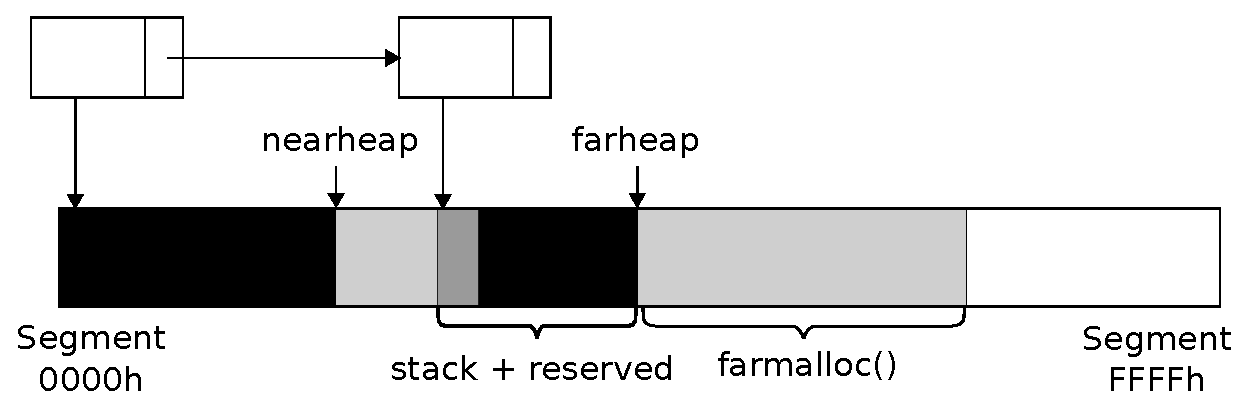
\includegraphics[width=\textwidth]{imgs/drawings/mm_stack.eps}
 \caption{Second locked block: stack.}
 \end{figure}
 \par

\par
Finally, the last unusable block of memory lies between the end of the far heap and the end of the 1MiB memory, the area that is typically for VRAM, ROM, etc. Now, the entire memory space from segment \cw{0000h} to \cw{FFFFh} is allocated, chained together, and fully controlled by the memory manager.\\

\begin{figure}[H]
\centering
 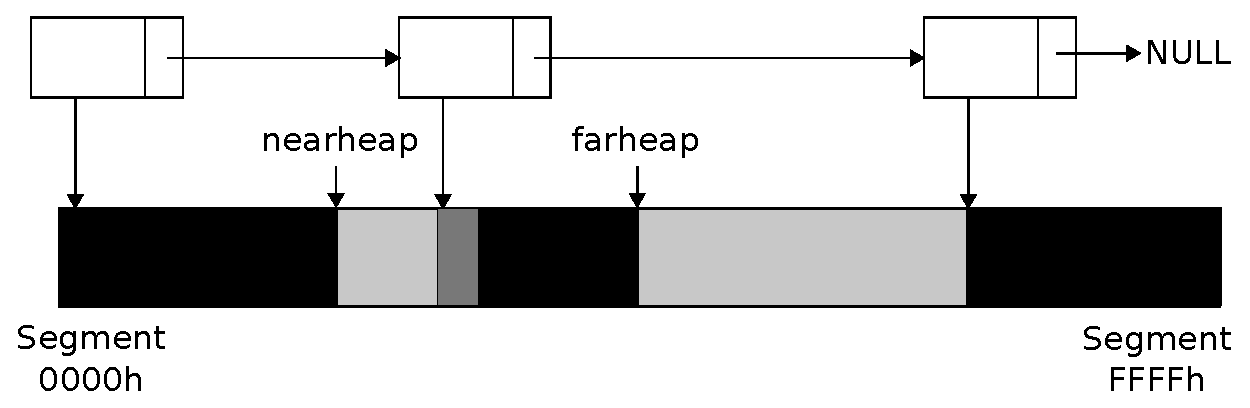
\includegraphics[width=\textwidth]{imgs/drawings/mm_final.eps}
 \caption{Final initial memory manager state.}
 \end{figure}

\par
The engine interacts with the Memory Manager by requesting RAM (\cw{MM\_GetPtr}) and freeing RAM (\cw{MM\_FreePtr}). To allocate memory, the manager searches for "holes" between
blocks\footnote{See the "Game Engine Black book Wolfenstein 3D" for a detailed description how the memory manager is allocating memory}. \\
\begin{figure}[H]
\centering
 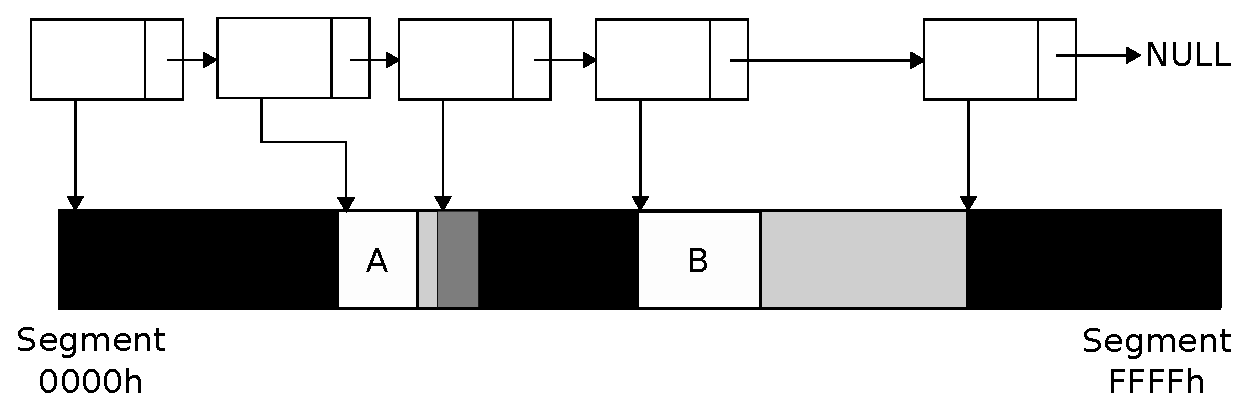
\includegraphics[width=\textwidth]{imgs/drawings/mm_allocation.eps}
 \caption{Allocation of memory.}
 \end{figure}
 \par

\par
By calling \cw{MM\_ShowMemory}, you can inspect the current memory usage during gameplay. Each pixel represents one memory segment of 16 bytes. Red indicates blocked memory, black indicates available memory, blue is unpurgeable memory, and purple is purgeable memory. Small white pixels indicate the start of new memory blocks in the linked list. Notice how small the near heap (the first black line) is compared to the far heap!\\

\begin{figure}[H]
	\centering
	\begin{subfigure}{1.0\linewidth}
		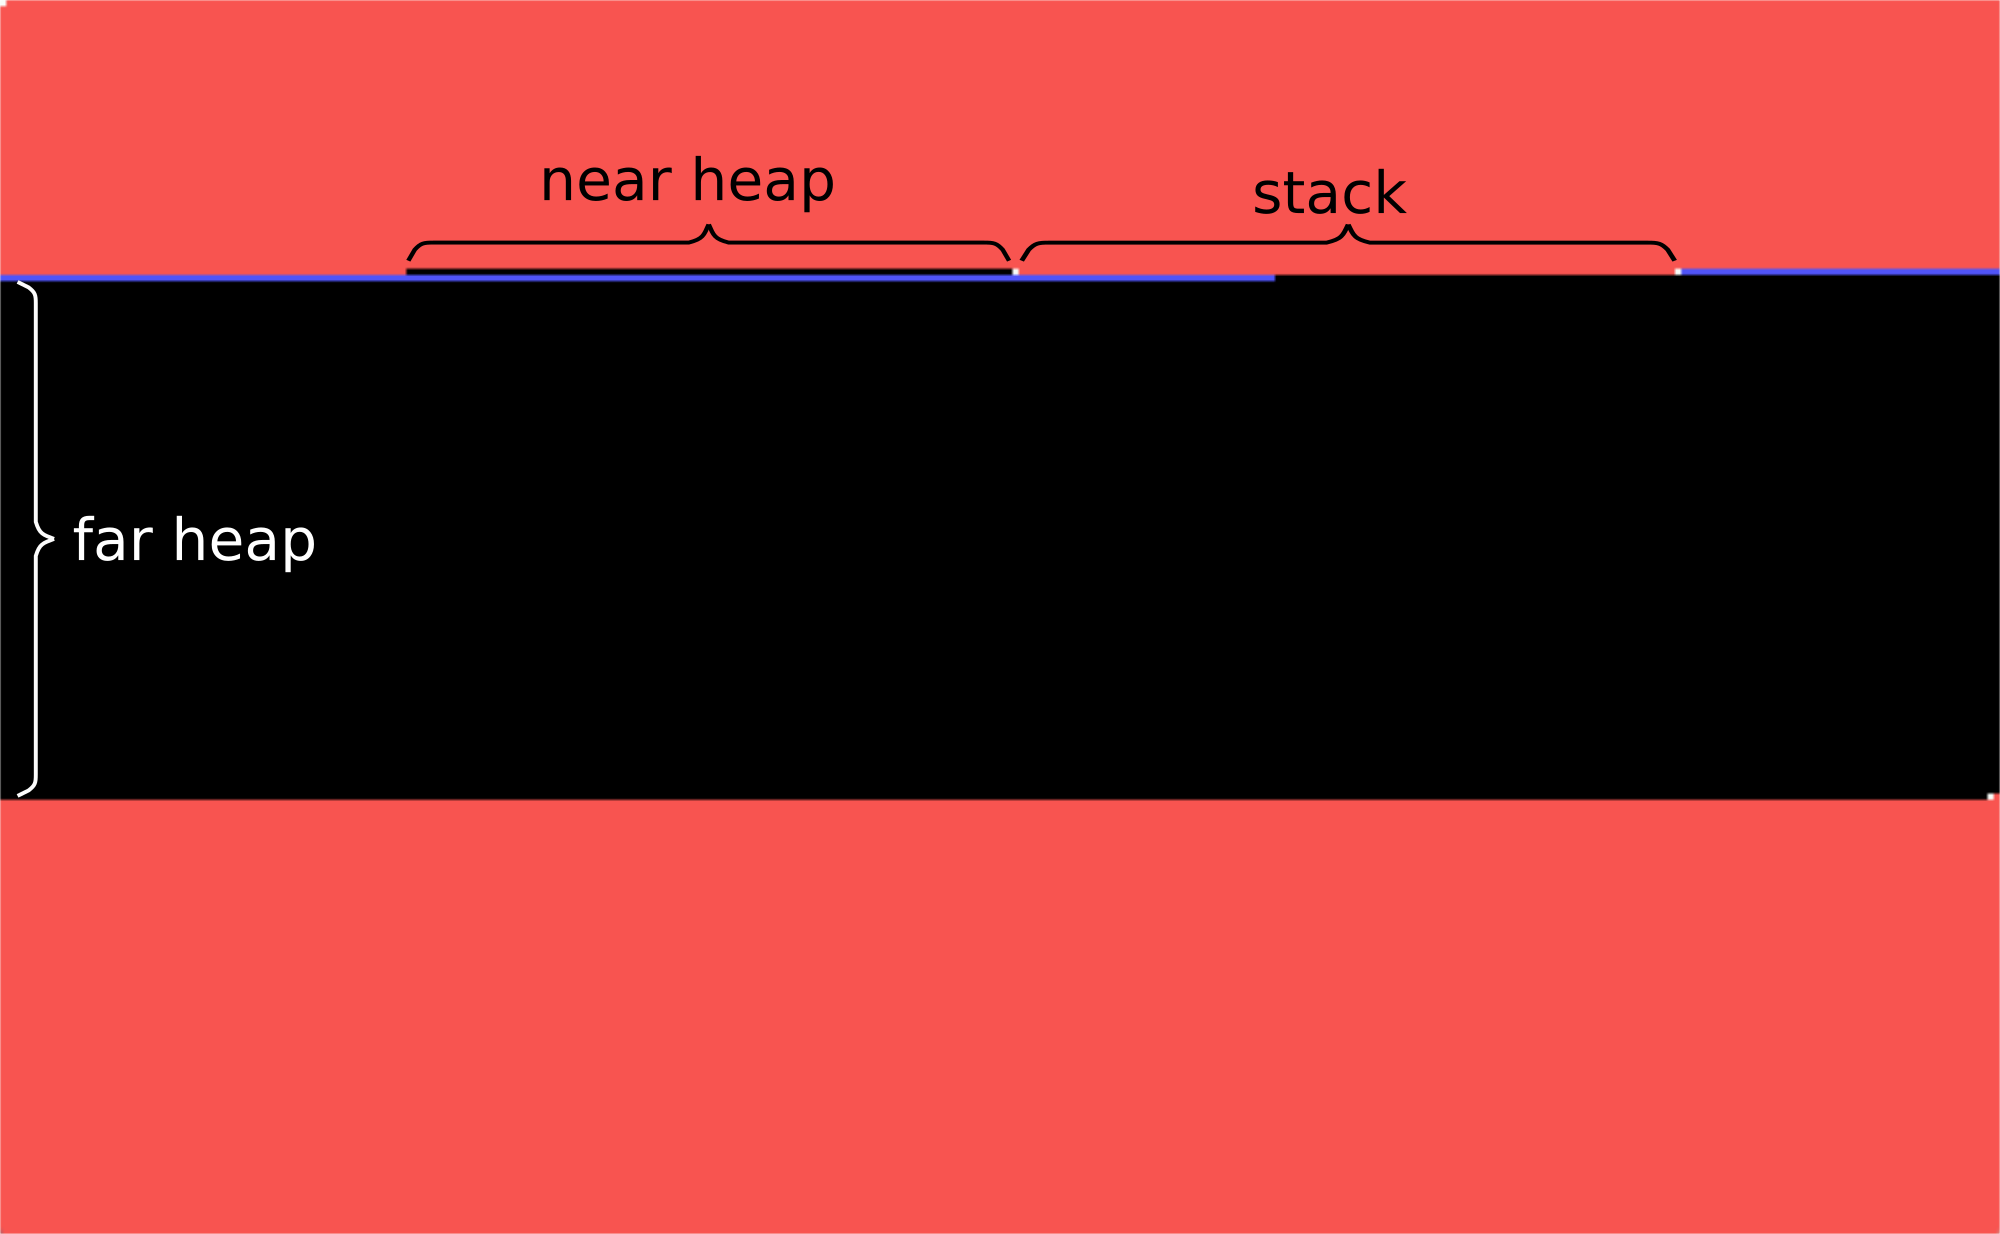
\includegraphics[width=\linewidth]{screenshots_300dpi/mm_dump_start_text.png}
	\end{subfigure}\\
	\vspace{3em}
	\begin{subfigure}{1.0\linewidth}
		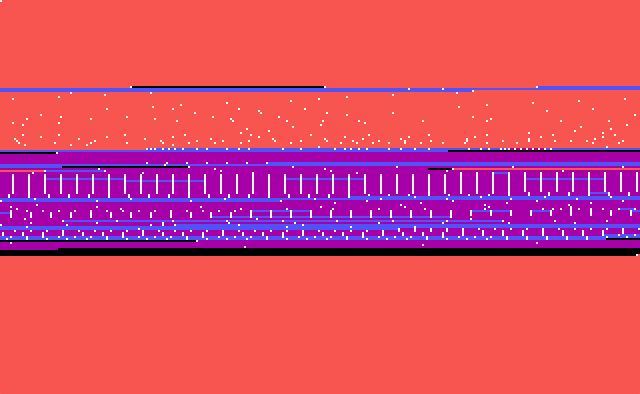
\includegraphics[width=\linewidth]{screenshots_300dpi/mm_dump_run.png}
	\end{subfigure}
	\caption{Memory dump after (i) initializing memory manager and (ii) running the game.}
	\label{fig:subfigures}
\end{figure}


\subsection{Video Manager (VW \& RF)}
The video manager features two parts:
\begin{itemize}
\item The \cw{VW\_*} layer is made of both C and ASM, where the C functions abstract away EGA register manipulation via assembly routines. 
\item The \cw{RF\_*} layer is used to refresh the screen, and is also made of both C and ASM code.
\end{itemize}
The video manager is described extensively in section \ref{section:adaptive_tile_refresh} on page \pageref{section:adaptive_tile_refresh}.

\subsection{Cache Manager (CA)}
The cache manager is a small but critical component. It loads and decompresses maps, graphics and audio resources stored on the filesystem and makes them available in RAM. Assets are stored into three files: 
\begin{itemize}
	\item A header file containing the offset to allow translation from asset ID to byte offset in the data file.
	\item A compression dictionary to decompress each asset.
	\item The data file containing the assets
\end{itemize}

\par
Details on each asset file are explained in Chapter \ref{section:programming}. The header and dictionary files are provided in the \cw{static} folder with the \cw{*.KDR} extension. These file types are integrated into the engine code and are required during compilation (converted into an \cw{*.OBJ} file using \cw{makeobj.c}). \\

\par
The data file containing the assets is not part of the source code and must be obtained by downloading the shareware version. All resources are compressed using Huffman compression, and maps have additional RLEW compression. The cache manager is described extensively in the "Asset Caching and Compression" section.\\

 \par
\begin{figure}[H]
\centering
 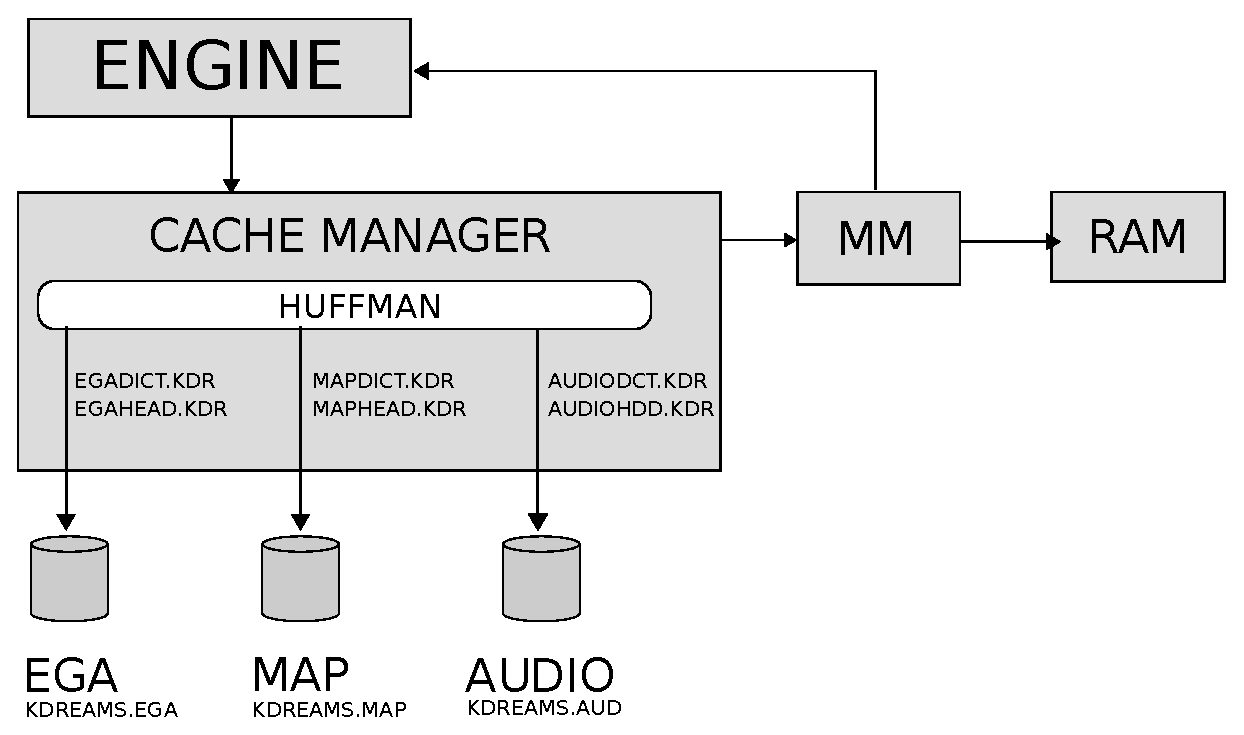
\includegraphics[width=\textwidth]{imgs/drawings/cache_manager_architecture.eps}
 \end{figure}




 
\subsection{User Manager (US)} 
\label{section:bitshifting}
The user manager is responsible for the layout of text and control panels, such as loading/saving games, configuring controls, and setting sound devices. Once we start the game, we move the display to EGA graphic mode \cw{0x0D}. Here we cannot print characters on the screen using the \cw{printf()} command. \\

\par
A key function of the user manager is to render text at a specific pixel location. When the engine needs to draw a string, it is passed to \cw{US\_Print} which does all measurement (\cw{VW\_MeasurePropString}) and then passes this information to \cw{VWB\_DrawPropString}, which takes care of drawing the string on screen.\\

\par
In the graphics asset file, each font character is stored with:
\begin{itemize}
  \item The width of the character
  \item The location in memory where each character is stored as a bitmap
\end{itemize}
Each character is 10 pixels tall, but the width varies, as illustrated in Figure \ref{fig:text_bitmap}. 
\begin{figure}[H]
\centering
 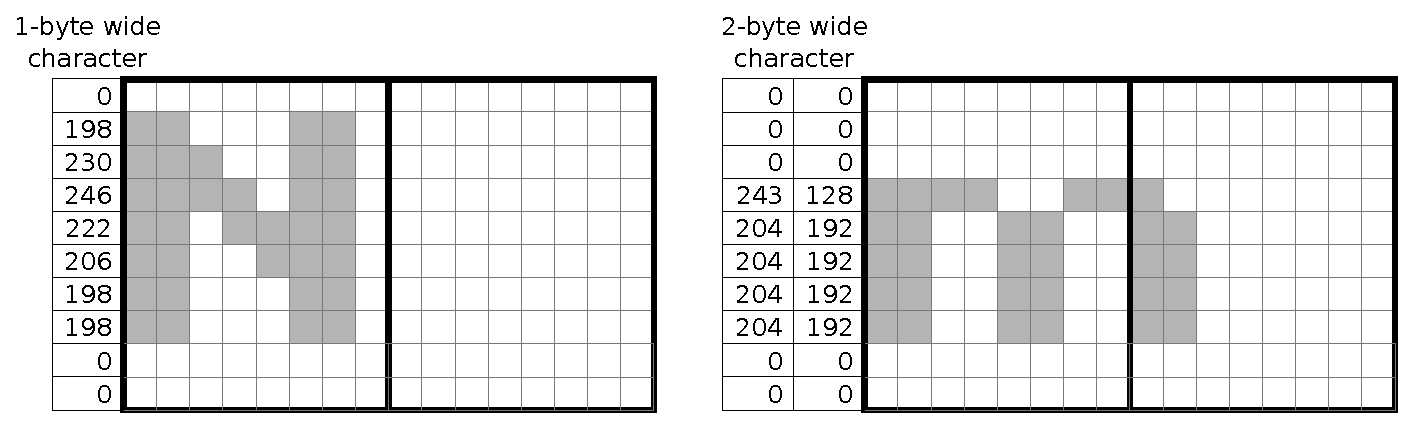
\includegraphics[width=\textwidth]{imgs/drawings/text_bitmap.eps}
 \caption{Character bitmaps of 'N' (7 bits wide) and 'm' (11 bits wide)}
 \label{fig:text_bitmap}
 \end{figure}
 \par
 
On the EGA videocard each 8 pixels take up 1 byte of VRAM (as explained in Section \ref{section:EGA_Planar_Madness} on page \pageref{section:EGA_Planar_Madness}). When you need to print characters that aren't perfectly aligned with this 8-pixel grid, how do you manage the alignment? Let's say you want to display the letter 'N' on the screen. If the 'N' starts in the middle of a byte (say at pixel 3 instead of pixel 0), you need a clever way to shift the bits over to ensure it appears correctly on the screen.\\

\par
Instead of manually shifting every pixel in your character bitmaps, the game engine uses pre-calculated bitshift tables. These tables are essentially lookup guides that help quickly adjust how characters are drawn based on their starting position. Here's how the process works:
\begin{enumerate}
  \item Start with a base table (called \cw{shiftdata0}) that holds all the possible values for a byte, from 0 to 255, and store this in an integer (16 bits). 
  \item Next, you generate seven more tables by shifting each value in \cw{shiftdata0} one bit to the right for each table. So for \cw{shiftdata1} the value 198 becomes 99, and for \cw{shiftdata2} it becomes 32817, and so on. This process continues until you have eight tables, each representing a different bitshift.
\end{enumerate}

\begin{figure}[H]
\centering
 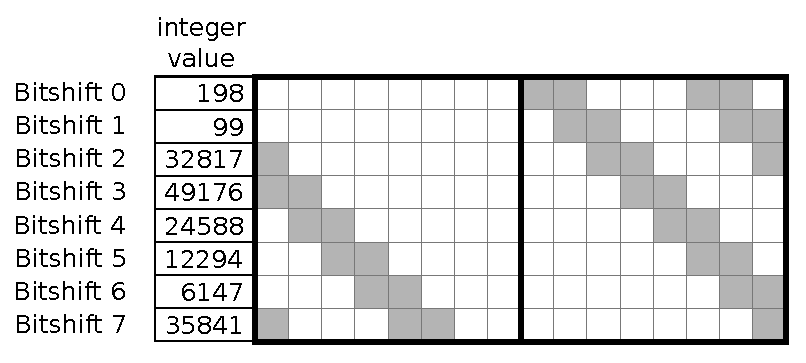
\includegraphics[width=0.8\textwidth]{imgs/drawings/shift_tables.eps}
 \caption{Right bitshift [0-7] for 198.}
 \label{fig:shiftttable}
 \end{figure}

\par
The pre-calculated bitshift table are stored in \cw{id\_vw\_a.asm}, below the \cw{bitshift3} table.\\

\begin{minipage}{\textwidth}
  \lstinputlisting[basicstyle=\fontsize{7}{9}\selectfont]{code/unrolled_shift_table.c}
\end{minipage}
\label{wallclip_array}

\par
Printing the letter "N" with an offset of 3 pixels involves a simple lookup in \cw{shiftdata3}, resulting in a 3-bit shifted "N" on the screen. By sacrificing a bit of memory, a lot of CPU time is saved. \\
\begin{figure}[H]
\centering
 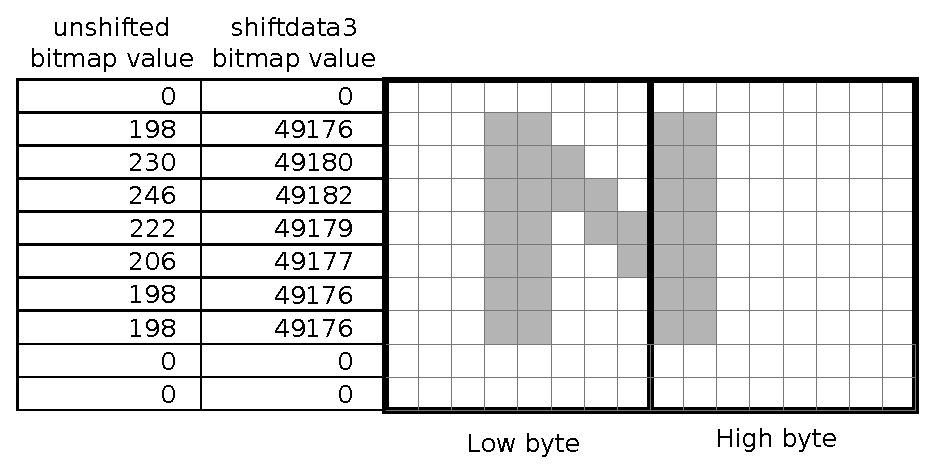
\includegraphics[width=0.8\textwidth]{imgs/drawings/text_bitshift_N.eps}
 \caption{Bitshift 'N' over 3 bits using bit shift tables.}
 \label{fig:text_bitshift_N}
 \end{figure}
 \par


\begin{minipage}{\textwidth}
  \lstinputlisting[language={[x86masm]Assembler}]{code/unrolled_ShiftPropChar.asm}
\end{minipage}
\par
\subsection{Sound Manager (SD)}
The Sound Manager abstracts interaction with all four sound systems supported: PC Speaker, AdLib, Sound Blaster, and Disney Sound Source. It is a beast of its own since it doesn't run inside the engine. Instead it is called via IRQ at a much higher frequency than the engine (the engine runs at a maximum 70Hz, while the sound manager ranges from 140Hz to 700Hz). \\
 \par
\begin{figure}[H]
\centering
 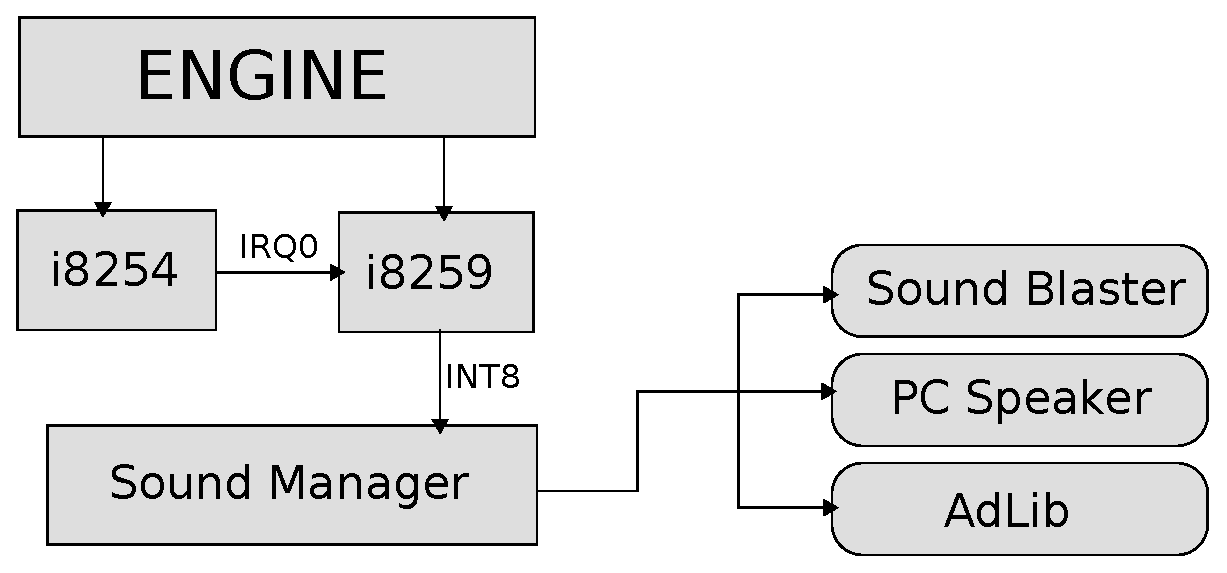
\includegraphics[width=\textwidth]{imgs/drawings/sound_manager_architecture.eps}
 \caption{Sound system architecture.}
 \end{figure}
 \par


\subsection{Input Manager (IN)}
The input manager abstracts interactions with joystick, keyboard, and mouse. It features the boring boilerplate code to deal with PS/2, Serial, and DA-15 ports, with each using their own I/O addresses.

\subsection{Softdisk files}
The primary function of the Softdisk files is to load and display the intro screen bitmap using the \cw{LoadLIBShape} function from soft.c. Most of the functions in these files are not used and are therefore not discussed further in this book.
\pagebreak



\section{Startup}
When the game engine starts, it first loads the Memory Manager. It then checks if at least 335KiB of RAM is available. If not, a warning is displayed, but the game can still continue. However, the game will likely crash or display an "Out of memory" error soon after. \\

\par
Once the game has successfully started, the intro image, a Deluxe Paint bitmap image (\cw{*.LBM}), is displayed. After the user presses any key, the intro image is unloaded from RAM to free up memory for runtime, and the control panel is displayed.\\

\begin{figure}[H]
\centering
\fullimage{Keen_intro_screen.png}
\caption{Keen Dreams intro screen}
\end{figure}
\pagebreak
\end{document}
